\begin{table}[!h]
	\centering
	\caption{Experimental results averaged over $n=10$ iterations (mean $\pm$ std. dev.).}
	\label{tab:results}
	\resizebox{\textwidth}{!}{%
		\begin{tabular}{c|ccc|c|cc|ccc}
			Dataset  & $B$ & $D$ & $D'$ & $\bar{S}_e$ & $\bar{\Lcal}_0$ & $\bar{\Lcal}_1$ & $c^*$ & $\bar{\Lcal}_0'$ & $\bar{\Lcal}_1'$  \\ \hline
			Polbooks & 3 & 3 & -- & $2.250 \pm 0.000$ & $0.563 \pm 0.042$ & $0.595 \pm 0.089$ & -- & -- & -- \\
			School & 10 & 13 & 10 & $1.894 \pm 0.004$ & $0.787 \pm 0.127$ & $0.885 \pm 0.129$ & $1.198 \pm 0.249$ & $0.793 \pm 0.132$ & $0.853 \pm 0.132$ \\
			FB egonet & 10  & 480 & 10 & $1.626 \pm 0.003$ & $1.326 \pm 0.043$ & $1.538 \pm 0.069$ & $0.94 \pm 0.019$ & $1.580 \pm 0.150$ & $1.605 \pm 0.106$
		\end{tabular}
	}
\end{table}

\begin{figure}[!h]
	\centering
	\begin{subfigure}[t]{0.28\linewidth}
		\centering
		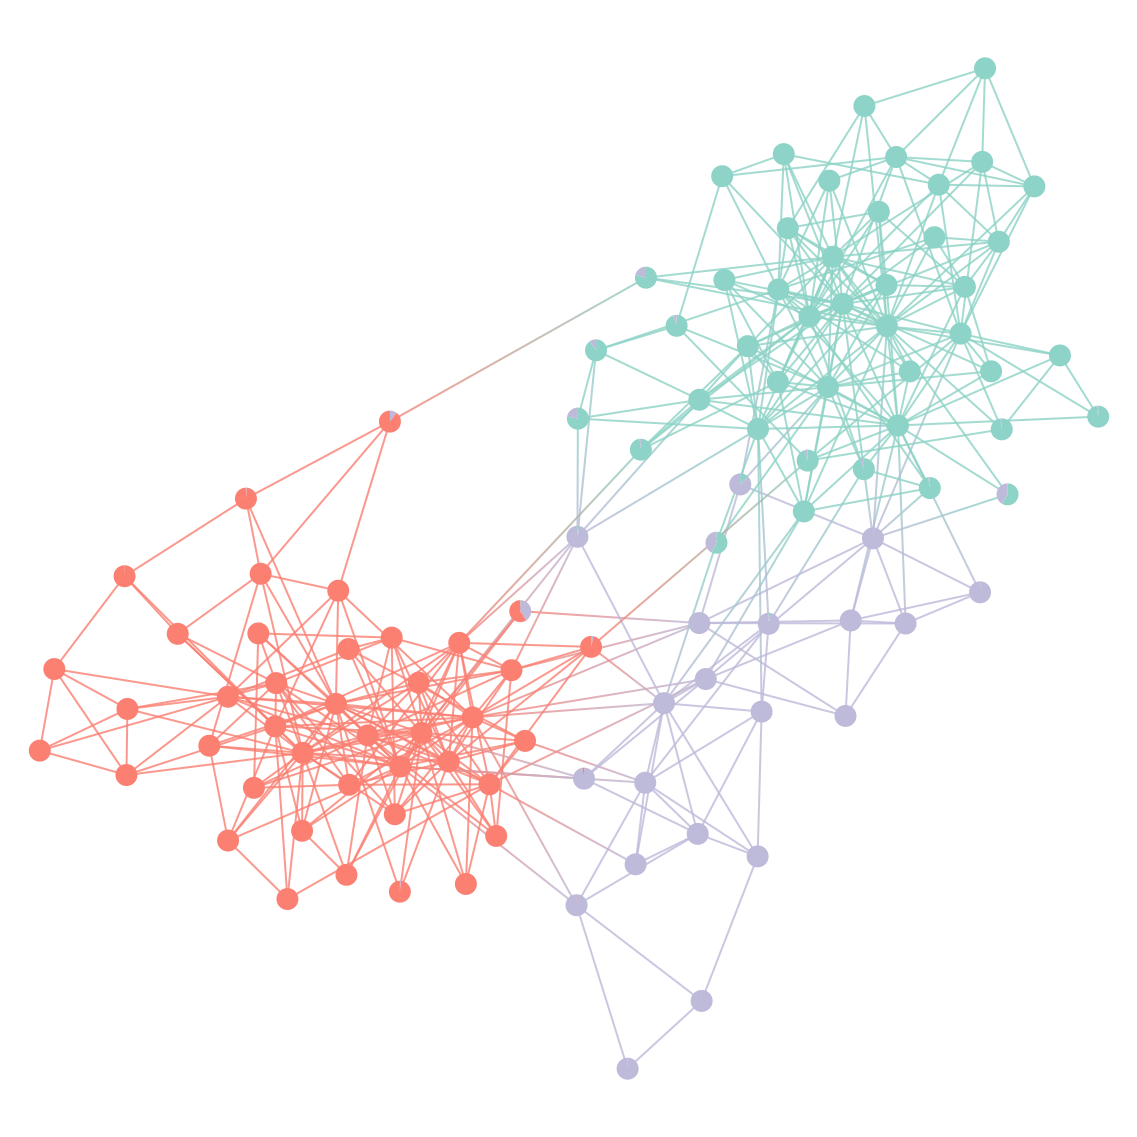
\includegraphics[width=\linewidth]{polbooks-graph.png}
		\caption{Polbooks}
		\label{fig:polbooks-graph}
	\end{subfigure}
	\hfill
	\begin{subfigure}[t]{0.28\linewidth}
		\centering
		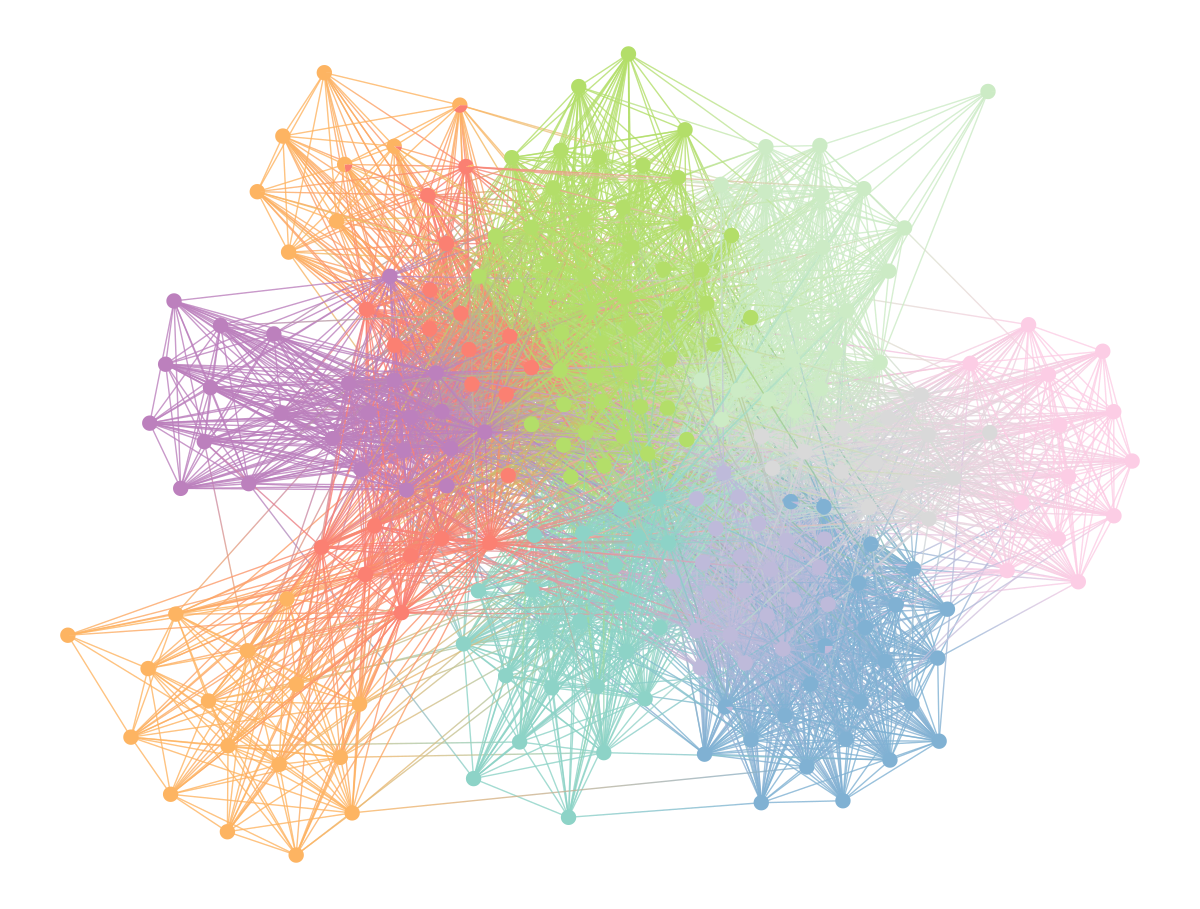
\includegraphics[width=\linewidth]{school-graph.png}
		\caption{School}
		\label{fig:school-graph}
	\end{subfigure}
	\hfill
	\begin{subfigure}[t]{0.28\linewidth}
		\centering
		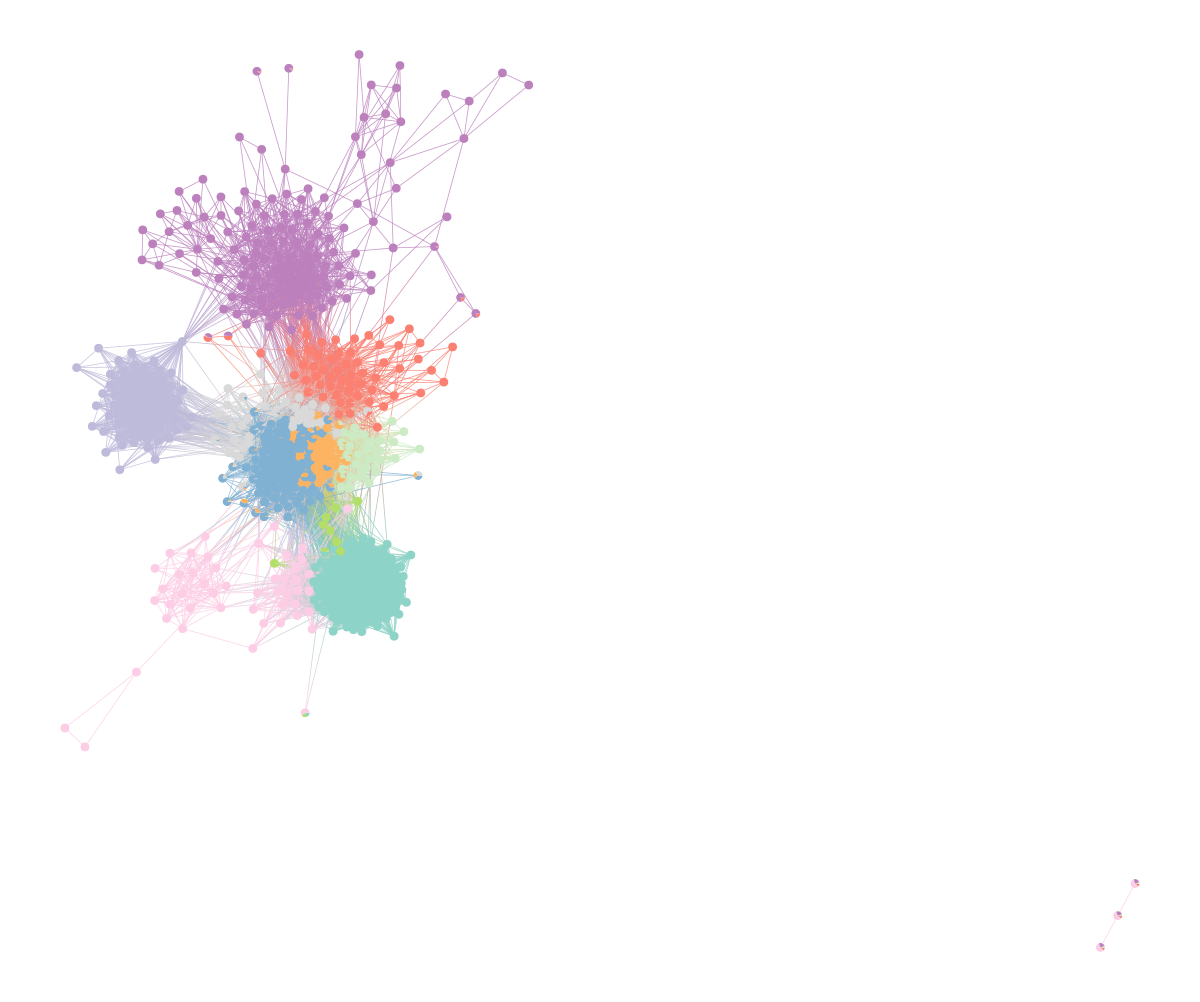
\includegraphics[width=\linewidth]{fb-graph.png}
		\caption{Facebook egonet}
		\label{fig:fb-graph}
	\end{subfigure}
	\begin{subfigure}[t]{0.11\linewidth}
		\centering
		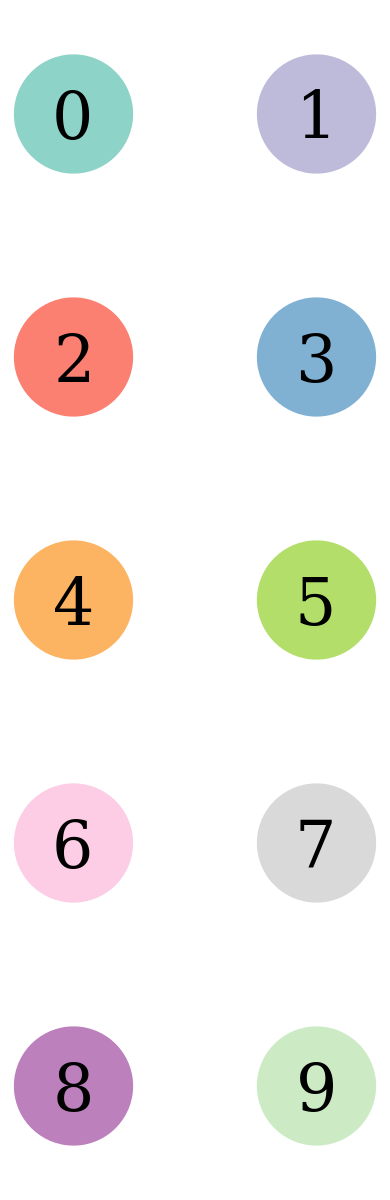
\includegraphics[width=0.8\linewidth]{10-vertical-legend.png}
		\caption{Block Legend}
		\label{fig:10-legend}
	\end{subfigure}
	\caption{Networks laid out and coloured according to inferred block memberships $\hat{y}$ for a given experiment iteration. Visualisation performed using \textit{graph-tool} \cite{peixoto_graph-tool_2014}.}
	\label{fig:graphs-all}
\end{figure}

\begin{figure}[!h]
	\centering
	\begin{subfigure}{0.32\linewidth}
		\centering
		\imagebox{0.9\linewidth}{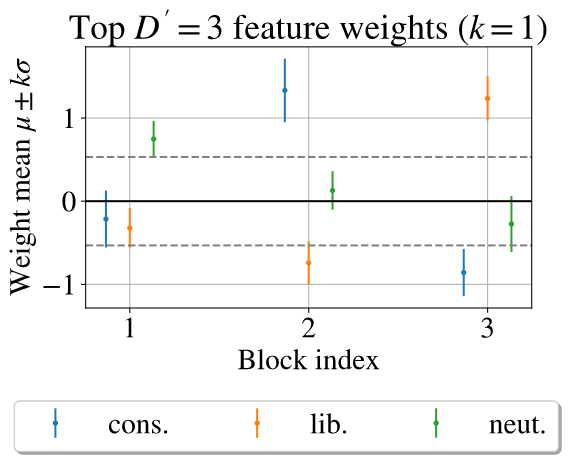
\includegraphics[width=\linewidth]{polbooks-null-1}}
		\caption{Political Books.}
		\label{fig:polbooks-null}
	\end{subfigure}
	\begin{subfigure}{0.32\linewidth}
		\centering
		\imagebox{0.9\linewidth}{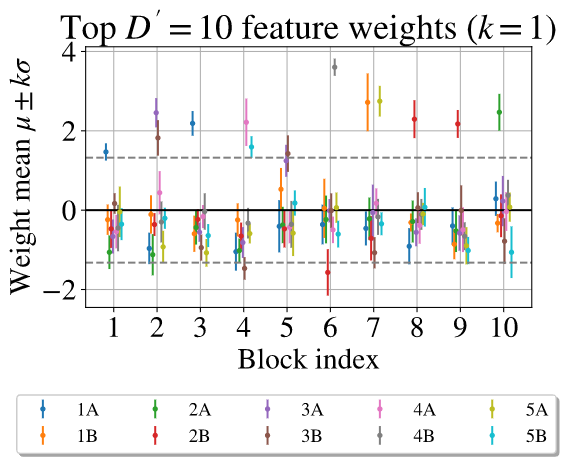
\includegraphics[width=\linewidth]{school-null-1}}
		\caption{Primary School.}
		\label{fig:school-null}
	\end{subfigure}
	\begin{subfigure}{0.32\linewidth}
		\centering
		\imagebox{0.9\linewidth}{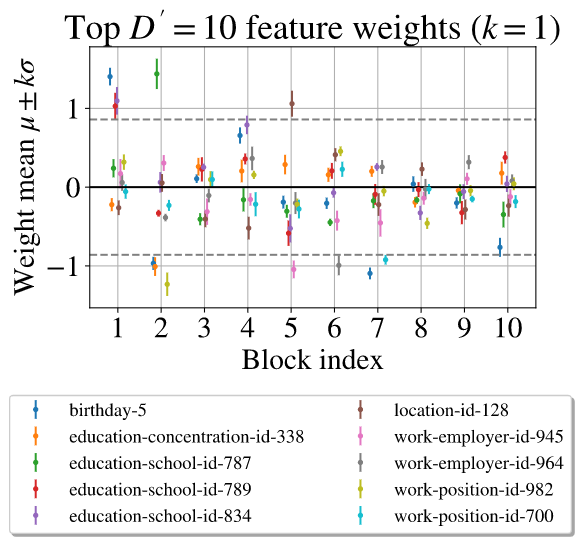
\includegraphics[width=\linewidth]{fb-null-1}}
		\caption{Facebook Egonet.}
		\label{fig:fb-null}
	\end{subfigure}
	\caption{$\theta$-samples. Dotted line $\pm c^*$.}
\end{figure}

\begin{figure}[!h]
	\centering
	\begin{subfigure}{0.32\linewidth}
		\centering
		\imagebox{0.8\linewidth}{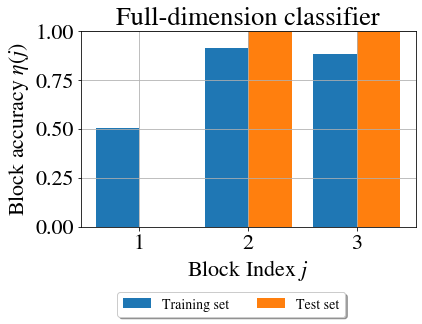
\includegraphics[width=\linewidth]{polbooks-accuracy-2}}
		\caption{Political Books.}
		\label{fig:polbooks-accuracy}
	\end{subfigure}
	\begin{subfigure}{0.32\linewidth}
		\centering
		\imagebox{0.8\linewidth}{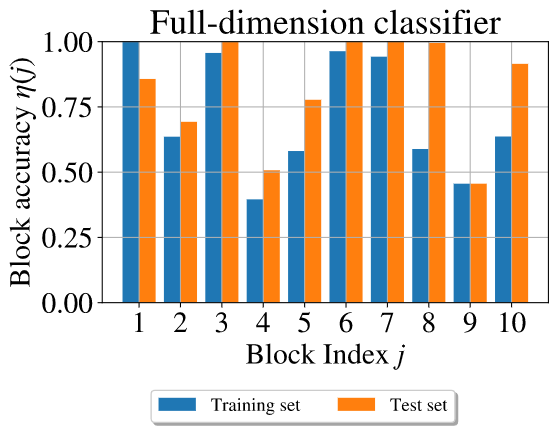
\includegraphics[width=\linewidth]{school-accuracy-1}}
		\caption{Primary School.}
		\label{fig:school-accuracy}
	\end{subfigure}
	\begin{subfigure}{0.32\linewidth}
		\centering
		\imagebox{0.8\linewidth}{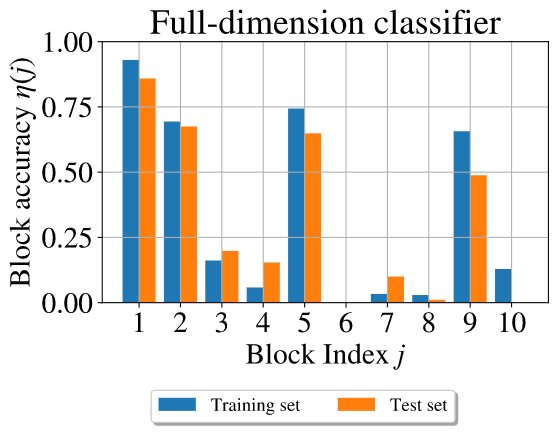
\includegraphics[width=\linewidth]{fb-accuracy-1}}
		\caption{Facebook Egonet.}
		\label{fig:fb-accuracy}
	\end{subfigure}
	\caption{Per-block accuracy $\eta(j)$.}
\end{figure}

% vertical layout takes up too much space
%\begin{figure}[!h]
%	\centering
%	\begin{minipage}{0.42\linewidth}
%		\centering
%		\begin{subfigure}{\linewidth}
%			\centering
%			\imagebox{0.8\linewidth}{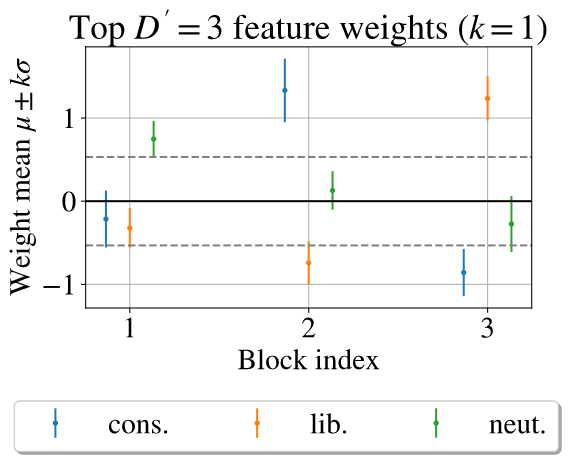
\includegraphics[width=\linewidth]{polbooks-null-1}}
%			\caption{Political Books.}
%			\label{fig:polbooks-null}
%		\end{subfigure}
%		
%		\begin{subfigure}{\linewidth}
%			\centering
%			\imagebox{0.85\linewidth}{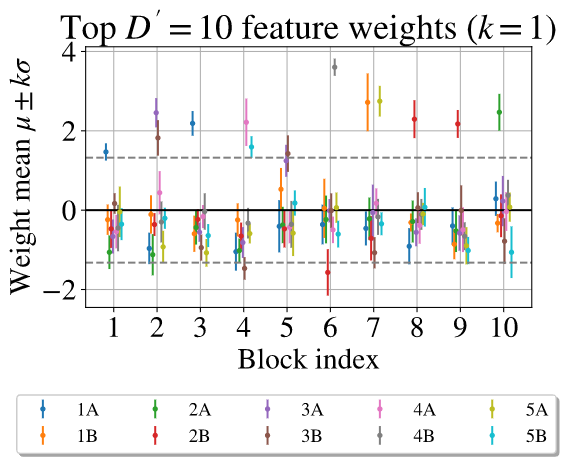
\includegraphics[width=\linewidth]{school-null-1}}
%			\caption{Primary School.}
%			\label{fig:school-null}
%		\end{subfigure}
%		
%		\begin{subfigure}{\linewidth}
%			\centering
%			\imagebox{0.9\linewidth}{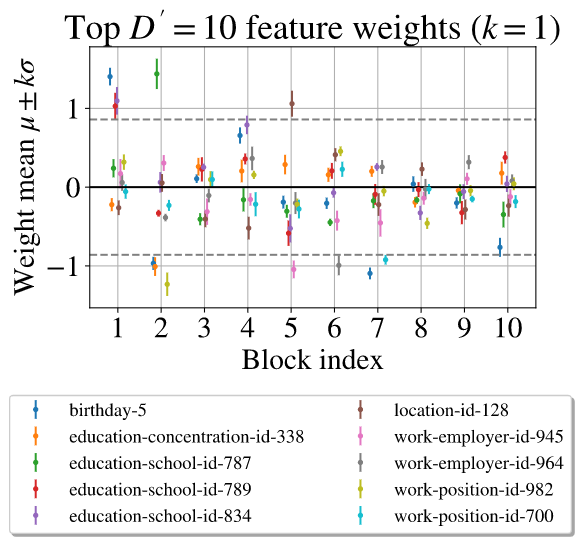
\includegraphics[width=\linewidth]{fb-null-1}}
%			\caption{Facebook Egonet.}
%			\label{fig:fb-null}
%		\end{subfigure}
%		\caption{$\theta$-samples. Dotted line $\pm c^*$.}
%	\end{minipage}
%	%
%	\begin{minipage}{0.42\linewidth}
%		\centering
%		\begin{subfigure}[t]{\linewidth}
%			\centering
%			\imagebox{0.8\linewidth}{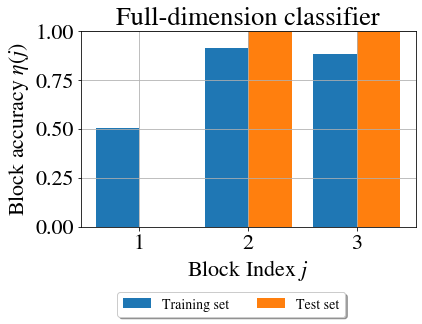
\includegraphics[width=\linewidth]{polbooks-accuracy-2}}
%			\caption{Political Books.}
%			\label{fig:polbooks-accuracy}
%		\end{subfigure}
%		
%		\begin{subfigure}{\linewidth}
%			\centering
%			\imagebox{0.85\linewidth}{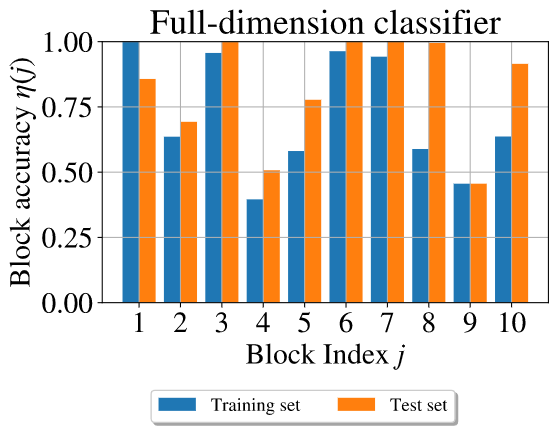
\includegraphics[width=\linewidth]{school-accuracy-1}}
%			\caption{Primary School.}
%			\label{fig:school-accuracy}
%		\end{subfigure}
%		
%		\begin{subfigure}{\linewidth}
%			\centering
%			\imagebox{0.9\linewidth}{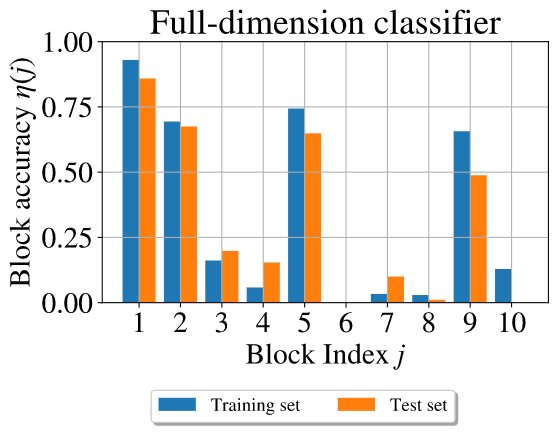
\includegraphics[width=\linewidth]{fb-accuracy-1}}
%			\caption{Facebook Egonet.}
%			\label{fig:fb-accuracy}
%		\end{subfigure}
%		\caption{Per-block accuracy $\eta(j)$.}
%	\end{minipage}
%\end{figure}